
\subsection{Abbildung des Organisationskontext}
Die Definition von Bilanzräumen, wie sie von Engelmann (2015, Kapitel 5.4.2) beschrieben wird, bildet eine wesentliche Grundlage für die Analyse und Optimierung der energiebezogenen Leistung von Organisationen. 
Dabei müssen die Bilanzraumkriterien den spezifischen Gegebenheiten der Organisation angepasst werden. Dies wird deutlich, wenn man den Energieverbrauch in verschiedenen Sektoren betrachtet.

\begin{figure}[H]
    \centering
    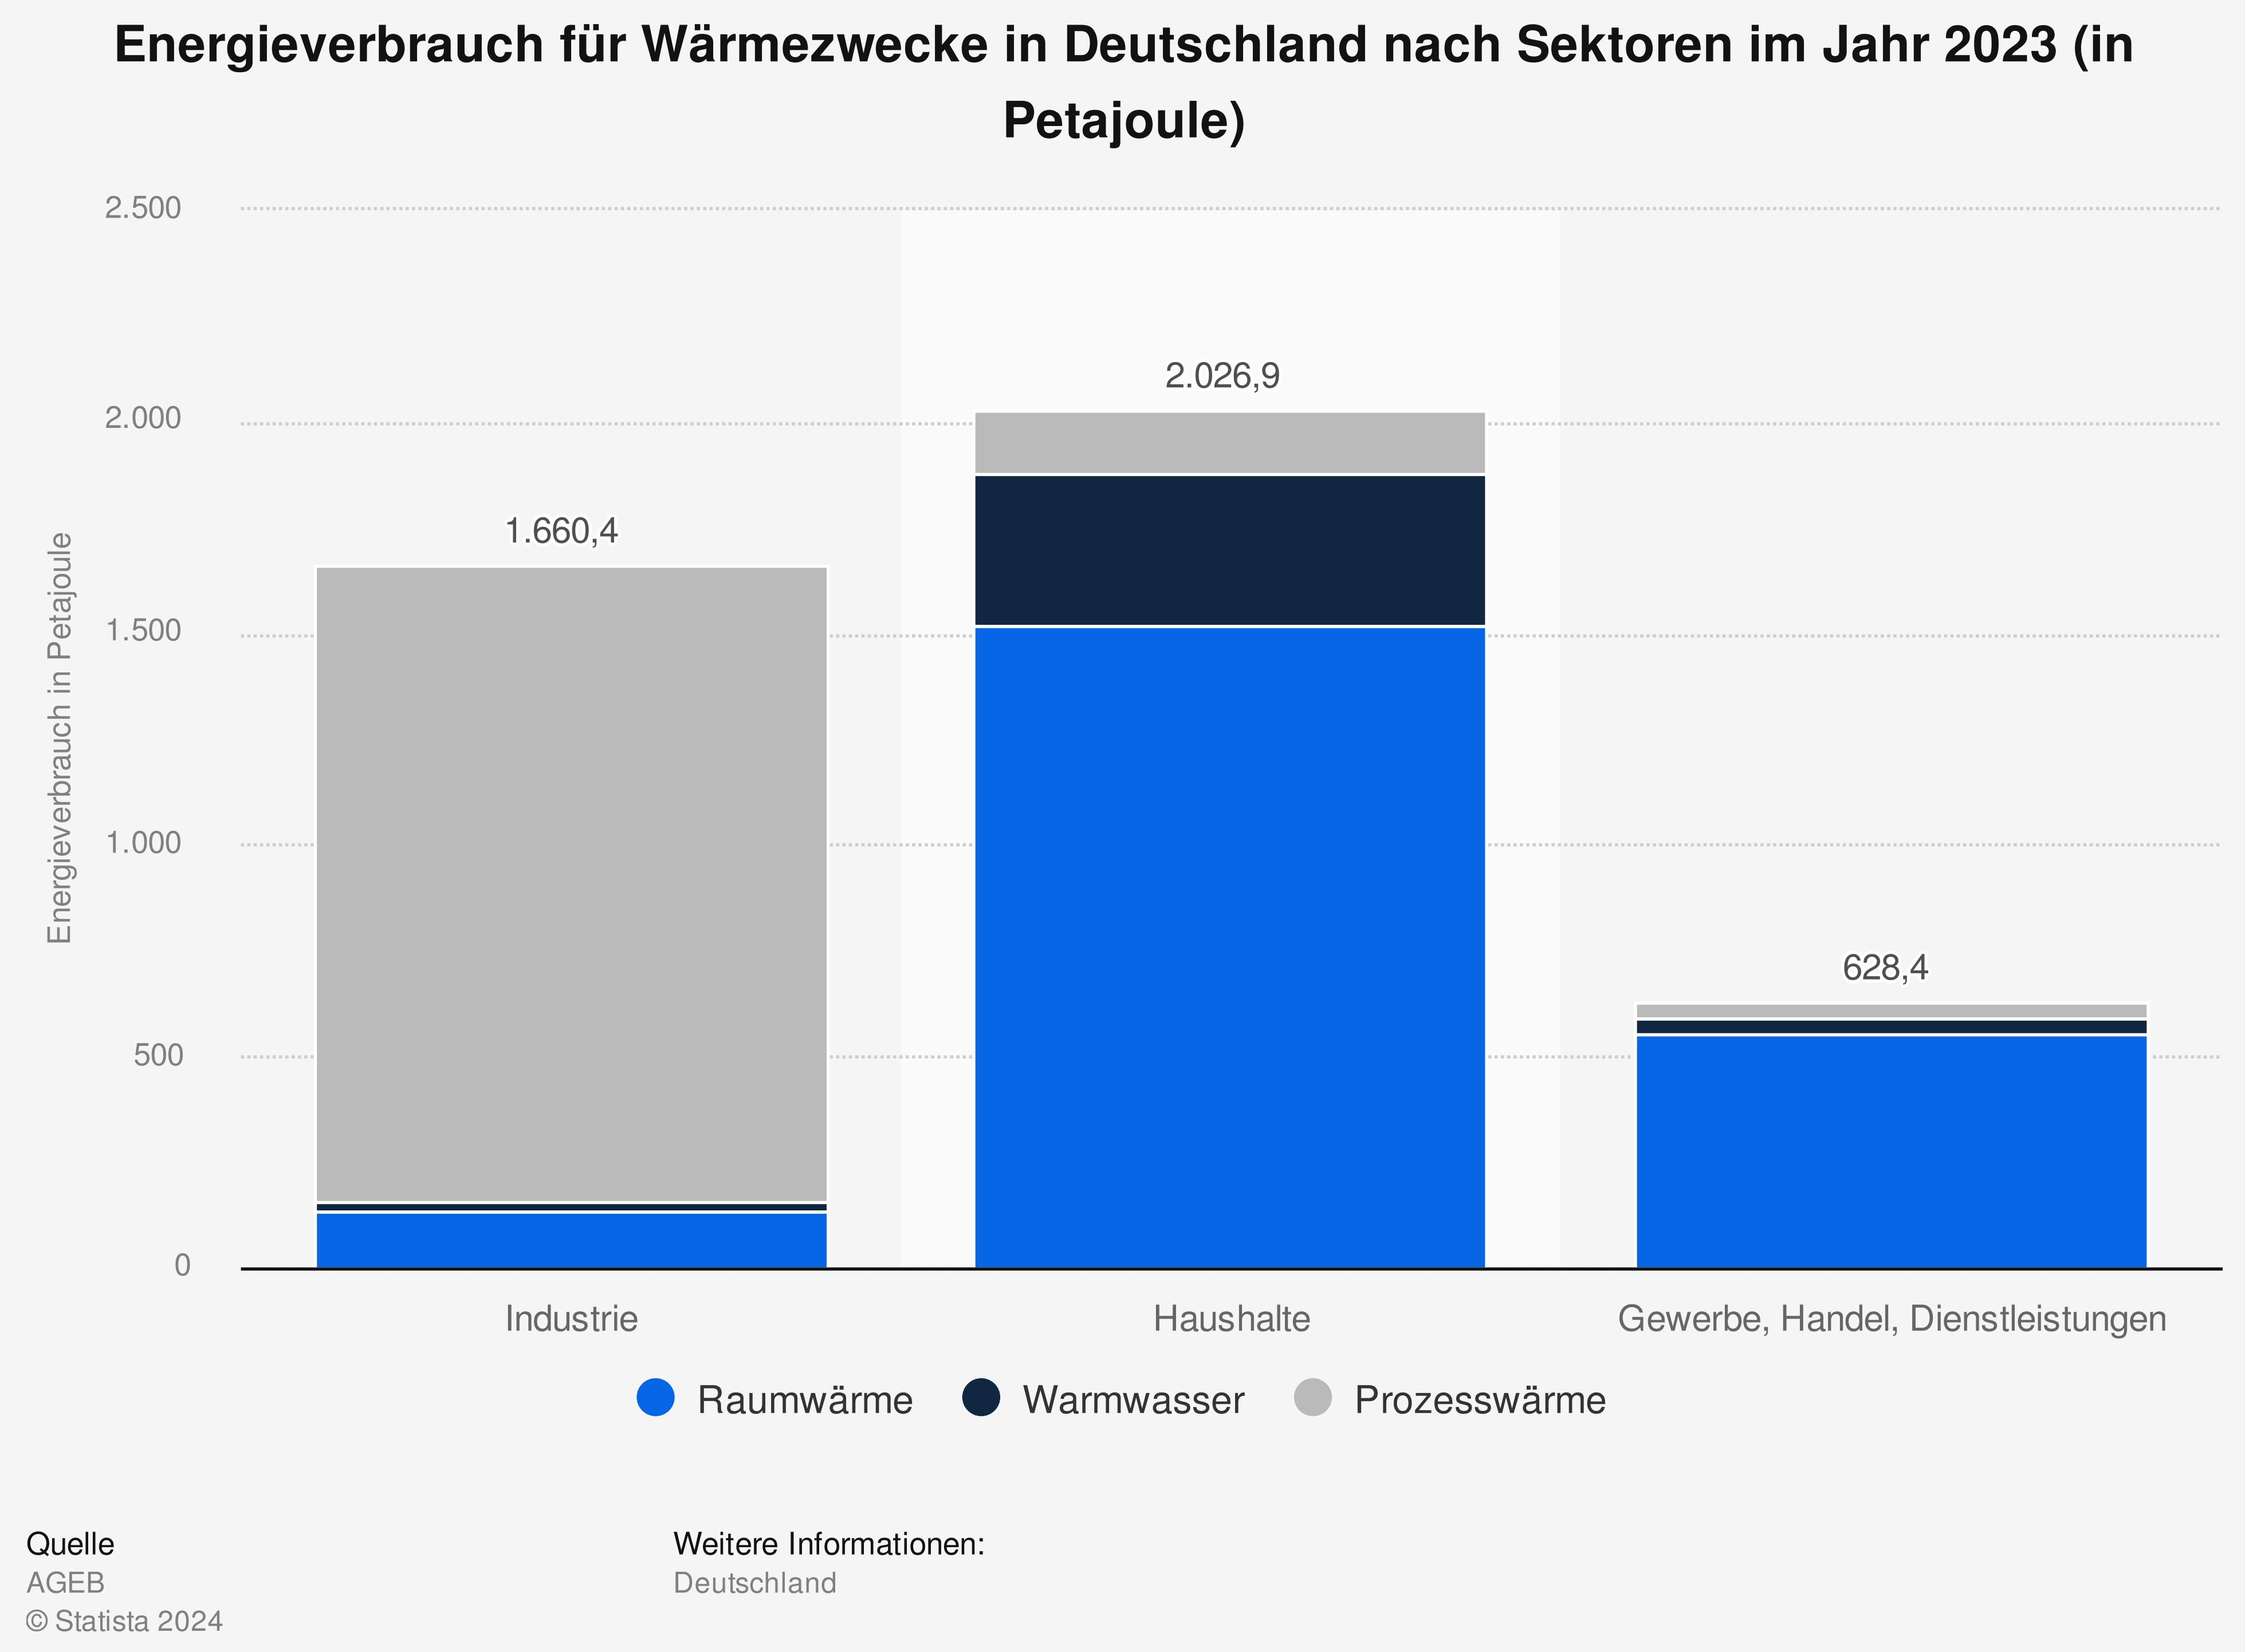
\includegraphics[width=1\textwidth]{../../Ressourcen/Bilder/Energieverbrauch_für_Wärmezweck_DE.jpg}
    \caption{Energieverbrauch für den Wärmezweck in Deutschland [\cite{AGEB.2024}]}
    \label{fig:Energieverbrauch_Wärme_DE}
\end{figure}

Abbildung \ref{fig:Energieverbrauch_Wärme_DE} zeigt den Energieverbrauch für Wärmezwecke in Deutschland im Jahr 2023, aufgeschlüsselt nach Sektoren. Hieraus lassen sich grundlegende Erkenntnisse für die 
praktische Definition von Bilanzräumen ableiten. Der industrielle Sektor weist einen hohen Anteil an prozessbezogener Wärme auf, was darauf hinweist, dass hier spezifische Bilanzräume für die Erfassung und 
Optimierung von Prozesswärme sinnvoll sind. Im Gegensatz dazu spielt im Dienstleistungssektor die Raumwärme eine dominierende Rolle denn in Organisationen, die immaterielle Dienstleistungen 
erbringen, spielt die Gebäudeenergie eine entscheidende Rolle bei der Verbesserung der energiebezogenen Leistung, während Prozesse oder Technologien eine untergeordnete Bedeutung haben [\cite{AlbertoFichera.2020}]. 
Dies erfordert andere Schwerpunkte bei der Definition von Bilanzraumkriterien.

Dieser Unterschied zeigt, dass ein einheitlicher Ansatz zur Definition von Bilanzraumkriterien sektorenübergreifend nicht zielführend ist. Stattdessen sollten die Bilanzraumkriterien auf den jeweiligen Energieeinsatz 
abgestimmt werden, um Optimierungspotenziale gezielt identifizieren zu können. Für Organisationen, die Dienstleistungen anbieten, bedeutet dies beispielsweise, dass die Gebäudeenergie als zentrale Energiesenke 
in den Fokus rückt, während bei Industriebetrieben die Energieflüsse innerhalb der Produktionsprozesse detaillierter bilanziert werden sollten.